% Final Year Project Final Report -- LaTeX replica (MAEG4999 style)
% Compile from this directory: pdflatex main.tex (twice for TOC)
\documentclass[12pt,a4paper]{report}

\usepackage[utf8]{inputenc}
\usepackage[T1]{fontenc}
\usepackage{lmodern}
\usepackage{microtype}
\usepackage[a4paper,margin=1in]{geometry}
% fancyhdr: avoid "headheight too small" warnings with 12pt body + header text
\setlength{\headheight}{14pt}
\addtolength{\topmargin}{-2pt}
\usepackage{setspace}
\setstretch{1.15}
% No first-line indent; separate paragraphs with vertical space (block style)
\usepackage{parskip}
\usepackage{fancyhdr}
\usepackage{graphicx}
\usepackage{booktabs}
\usepackage{array}
\usepackage{tabularx}
\usepackage{longtable}
\usepackage{amsmath,amssymb}
% IEEE-style numeric citations (compression, sorting); load before hyperref
\usepackage{cite}
% Allow line breaks in long DOI URLs (references.bib url={https://doi.org/...})
\usepackage[hyphens]{url}
\usepackage[hidelinks]{hyperref}

% Figure path: project results folders. Build: docs/latex/compile.sh → docs/final_report.pdf
\graphicspath{{../../results/figures/binary/}{../../results/figures/multiclass/}{../../results/figures/pipeline/}}
% Tall MATLAB figures (confusion + pipeline): cap height so nothing is clipped at page bottom
\newcommand{\includegraphicsresult}[1]{%
  \includegraphics[width=0.92\linewidth,height=0.68\textheight,keepaspectratio]{#1}}

\pagestyle{fancy}
\fancyhf{}
% Short header text avoids two-line headers on dense literature pages
\fancyhead[C]{\small MAEG4999 FYP II --- Robotic Exoskeleton for Load Transportation}
\fancyfoot[C]{\thepage}
\renewcommand{\headrulewidth}{0.4pt}
\fancypagestyle{plain}{%
  \fancyhf{}
  \fancyfoot[C]{\thepage}
  \renewcommand{\headrulewidth}{0pt}
}

\hypersetup{
  pdftitle={Robotic Exoskeleton for Load Transportation - Final Report},
  pdfauthor={Yim Fu Chong}
}

% Numeric results synced with results/metrics/*/*.mat — regenerate via scripts/ExportMetricsForReport.m
% AUTO-GENERATED — do not edit by hand.
% Regenerate: scripts/ExportMetricsForReport.m
% Source: results/svm_evaluation_metrics_*.mat, multiclass_evaluation_metrics.mat
\newcommand{\BinaryOofAccUsc}{98.91}
\newcommand{\BinaryOofAccHuGa}{88.60}
\newcommand{\BinaryOofAccMerged}{94.50}
\newcommand{\MulticlassOofAcc}{56.76}
% Optional: run TrainLstmBinary + EvaluateLstmConfusion, then re-export.
\newcommand{\HasLstmMetrics}{0}


\begin{document}

% ---------- Roman front matter ----------
\pagenumbering{roman}

\begin{titlepage}
  \centering
  \vspace*{1.5cm}
  {\large WHL3.}\\[1.2cm]
  {\LARGE \textbf{Robotic Exoskeleton for Load Transportation}}\\[1.5cm]
  By: Yim Fu Chong (1155176974)\\[0.8cm]
  Supervisor: Professor Wei-Hsin Liao\\[1.5cm]
  {\large Final Year Project Final Report}\\[0.6cm]
  Submitted in Partial Fulfillment of the\\
  Requirements for\\[0.5cm]
  The Degree of Bachelor of Engineering\\[0.8cm]
  Department of Mechanical and Automation Engineering\\
  The Chinese University of Hong Kong\\[1.5cm]
  {\large \today}
  \vfill
\end{titlepage}

\chapter*{Acknowledgments}
\addcontentsline{toc}{chapter}{Acknowledgments}
I would like to express my sincere gratitude to my supervisor Professor Wei-Hsin Liao. His insights into robotic exoskeletons and actuation systems have been instrumental in shaping the direction and progress of my work.

I am also deeply thankful to the team at ExoTechHK Limited for their collaboration and providing access to their lower-limb exoskeleton prototype. This partnership, facilitated under the Hong Kong Science and Technology Parks (HKSTP) incubation programme, has offered a practical pathway for technology transfer and real-world application.

Special thanks go to the Department of Mechanical and Automation Engineering at The Chinese University of Hong Kong for the resources and facilities that enabled this research. Additionally, I appreciate the contributions from fellow researchers and peers who provided feedback during the development phase.

Finally, I extend my appreciation to my family and friends for their encouragement and understanding during this challenging yet rewarding endeavor.

\begin{flushright}
Yim Fu Chong\\
\today
\end{flushright}

\chapter*{Abstract}
\addcontentsline{toc}{chapter}{Abstract}
\subsection*{Objectives}
This project develops a software-centric control-supervision module for a lower-limb robotic exoskeleton intended to assist heavy load transportation tasks ($>20$~kg) in industrial, logistics, and construction settings. The focus of the submitted work is real-time locomotion-intent recognition from inertial measurement unit (IMU) data, stable assist gating, and reproducible MATLAB-based evaluation on public datasets.

\subsection*{Methods}
The validated MATLAB baseline uses overlapping IMU windows of 100 samples at 100~Hz with a 50-sample step. Kalman fusion (\texttt{imufilter}) is included for simulation-side kinematic visualization rather than as mandatory classifier preprocessing.

The primary deployment classifier is a binary RBF support vector machine trained on a 30-dimensional handcrafted feature vector: five statistics per IMU slot across six slots. The final pipeline is centered on HuGaDB and uses a protocol-aware streaming policy with quality gating and official gyro-corruption handling. USC-HAD is retained as a separate benchmark dataset under the same feature layout. Binary labels group activities into active movement versus inactive movement for assist gating.

For analysis beyond binary gating, the repository also includes dataset-native multiclass ECOC models and optional sequence-based LSTM baselines. Binary and multiclass LSTM models operate on feature-by-time IMU sequences and are evaluated separately from the SVM baselines. Assist decisions in replay are stabilized by a finite-state machine with asymmetric hysteresis: three consecutive active predictions to engage assistance and five consecutive inactive predictions to release it.

\subsection*{Results}
Binary SVM five-fold out-of-fold accuracy from the committed evaluation outputs is \textbf{\BinaryOofAccUsc\%} on USC-HAD and \textbf{\BinaryOofAccHuGa\%} on HuGaDB under the multi-activity streaming policy. Native multiclass SVM accuracies on stratified subsamples are \textbf{\MulticlassOofAccUsc\%} on USC-HAD and \textbf{\MulticlassOofAccHuGa\%} on HuGaDB.

\ifnum\HasBinaryLstmMetrics=1
Binary LSTM holdout accuracy is \textbf{\LstmBinaryHoldoutAccUsc\%} on USC-HAD and \textbf{\LstmBinaryHoldoutAccHuGa\%} on HuGaDB.
\else
Binary LSTM metrics are optional and are exported after running the dataset-specific LSTM evaluation scripts.
\fi
\ifnum\HasMulticlassLstmMetrics=1
Native multiclass LSTM holdout accuracy is \textbf{\LstmMulticlassHoldoutAccUsc\%} on USC-HAD and \textbf{\LstmMulticlassHoldoutAccHuGa\%} on HuGaDB.
\else
Multiclass LSTM metrics are optional and are exported after running the dataset-specific sequence-model evaluation scripts.
\fi

Pseudo-real-time replay on held-out HuGaDB sessions shows that the combined classifier and FSM pipeline produces a stable binary assist command alongside IMU magnitude for visualization context. This report \textbf{emphasizes} the \textbf{multiclass LSTM} pseudo-real-time replay on HuGaDB subject~\ReplayHuGaDBSubject{}, session~\ReplayHuGaDBSession{} as the principal sequence-model demonstration: native twelve-class predictions over time on the same held-out session used for the binary replay figures.

\subsection*{Conclusions}
The project delivers a reproducible HuGaDB-centered MATLAB baseline for exoskeleton assist gating, with traceable scripts, saved metrics, evaluation figures, and replay outputs. The strongest validated \emph{classification} headline remains the binary SVM under the HuGaDB streaming policy, while the multiclass LSTM replay (subject~\ReplayHuGaDBSubject{}, session~\ReplayHuGaDBSession{}) is highlighted as the end-to-end sequence-model visualization for fine-grained activity behavior. Multiclass SVM and additional LSTM holdout metrics remain supporting analyses alongside that emphasis. The resulting software pipeline provides a solid foundation for future hardware integration, embedded deployment, and controlled experimental studies.


\tableofcontents
\clearpage

% ---------- Main body ----------
\pagenumbering{arabic}
\setcounter{page}{1}

\chapter{Problem Description}

\section{Problem Statement}
Manual load transportation in industrial, construction, and logistics settings frequently involves carrying loads exceeding 20~kg, surpassing human physiological limits and leading to high rates of lower-back pain, musculoskeletal disorders (MSDs), reduced productivity, and billions in annual economic costs worldwide. Existing assistive exoskeletons often fail to provide proactive, real-time adaptation to the user's locomotion intent or environmental changes, resulting in delayed or mismatched assistance that compromises safety and comfort. Moreover, generic assistance profiles do not account for inter-individual differences in gait asymmetry, fatigue thresholds, anthropometrics, or preferred movement patterns. These limitations are especially critical in dynamic workplaces where load magnitude, terrain, and tasks constantly vary. There remains a clear need for a lightweight, cost-effective lower-limb exoskeleton that delivers accurate intent detection, robust sensor fusion, and truly personalized adaptive control---without relying on invasive interfaces such as electromyography (EMG) or requiring extensive user training.

\section{Project Goal}
The primary goal is to develop a software-centric enhancement module for ExoTechHK Limited's existing lower-limb exoskeleton prototype---a local startup incubated at HKSTP and founded by CUHK researchers---to augment human strength and endurance during heavy load-carrying tasks ($>20$~kg) without invasive sensors or lengthy calibration.

\subsection*{Implemented scope}
The module integrates two core components as realized in code:
\begin{itemize}
  \item \textbf{Data acquisition and processing:} \textbf{HuGaDB} deployment path; held-out HuGaDB replay for pseudo-real-time testing; optional Kalman visualization (\texttt{imufilter}); \textbf{binary} RBF SVM on HuGaDB 30-D window features with USC-HAD / HuGaDB benchmark comparisons retained for the paper and poster; optional \textbf{native ECOC} SVMs (twelve USC-HAD / twelve HuGaDB activity classes); optional \textbf{binary and multiclass LSTM} sequence models on per-dataset IMU windows (\texttt{TrainLstmBinary}, \texttt{TrainLstmMulticlass}, \texttt{RunExoskeletonPipelineLstm}). Embedded deployment remains future work.
  \item \textbf{Binary active-movement intent:} Labels map activity to \textbf{active movement} vs.\ \textbf{inactive}. The final pipeline trains on the HuGaDB binary SVM path, while public-dataset comparison and replay-based simulation remain separate supporting workflows. The optional LSTM uses a 20\% holdout metric rather than five-fold OOF.
\end{itemize}

Being entirely software-based, the solution enables seamless integration into existing hardware prototypes, rapid deployment, and scalability across future platforms.

\section{Significance of the Project}
This project directly addresses a major occupational health challenge affecting industrial workers, logistics and construction personnel, and military operators exposed to heavy manual handling. In Hong Kong, manual handling injuries are a leading cause of absenteeism and healthcare expenditure. By providing proactive, personalized torque assistance at the hips and knees using cooperative control strategies---in which the exoskeleton follows rather than leads the user---the system aims for high accuracy in intent detection; recent field evidence shows that such user-following approaches improve usability compared to fixed profiles~\cite{le2024}.

Conducted in close collaboration with ExoTechHK Limited under the HKSTP incubation programme, the project offers a pathway for technology transfer and commercialization. Software-centric design enables low-cost retrofitting to existing lower-limb platforms and upgrades across hardware generations, with potential to broaden adoption. The technology aligns with United Nations Sustainable Development Goal 8 (Decent Work and Economic Growth) and strengthens Hong Kong's innovation ecosystem through industry--academia partnership. The reproducible HuGaDB training and held-out replay protocol supports repeatable evaluation without relying on project-specific phone recordings.

% Chapter 2 -- mirrors PDF structure and content (condensed where noted)
\chapter{Background Knowledge and Literature Review}

\section{Introduction}
The literature review focuses on existing research related to robotic exoskeletons for back support, particularly in the context of manual material handling (MMH) and load transportation tasks. Key themes include exoskeleton designs (passive vs.\ active, rigid vs.\ flexible), actuation systems (with emphasis on cable-driven and series elastic actuators), control strategies (including intention detection, sensor fusion, and machine learning), and personalization mechanisms. The review draws from systematic reviews, empirical studies, and technical papers to identify advancements, limitations, and gaps relevant to the project's goal of developing a software-centric enhancement module for a lower-limb exoskeleton. To provide a comprehensive overview, this review incorporates recent systematic analyses from 2020--2025, highlighting post-pandemic advancements in hybrid designs, AI integration, and industrial evaluations. For instance, Pesenti et al.~\cite{pesenti2021} and subsequent updates in Kermavnar et al.~\cite{kermavnar2021} and later works in bioengineering reviews classify over 30 back-support exoskeletons, emphasizing the shift toward soft and quasi-passive systems for improved user acceptance.

\section{Overview of Back-Support Exoskeletons for MMH}
Back-support exoskeletons (BSEs) are designed to mitigate low back pain and musculoskeletal disorders (MSDs) associated with repetitive lifting, bending, and load carrying in industries such as construction, logistics, and manufacturing. A systematic review by De Looze et al.~\cite{delooze2016} and updated analyses by Pesenti et al.~\cite{pesenti2021} classify BSEs into passive and active types. Passive BSEs, such as the Laevo or SPEXOR, rely on mechanical springs or elastic bands to store and release energy during trunk flexion-extension (TFE) motions, reducing erector spinae muscle activity by 10--40\% without requiring power sources. However, they offer limited adaptability to dynamic tasks and may impose resistance during non-assisted movements.

Recent evaluations, such as Luger et al.~\cite{luger2023}, evaluated the Laevo V2 passive exoskeleton in male workers and reported 12--19\% lower erector spinae activity during symmetric and asymmetric static holding tasks. Koopman et al.~\cite{koopman2020} further quantified that although passive exoskeletons effectively reduce peak L5/S1 moments during symmetric lifting, the moment reduction diminishes significantly when lifting involves trunk rotation or asymmetry---reinforcing the need for active, adaptive systems in real-world industrial settings where perfectly symmetric lifts are rare.

Active BSEs, like the SuitX BackX or Ekso Bionics' EksoVest, incorporate powered actuators to provide on-demand assistance, achieving up to 50\% reduction in metabolic cost and lumbar compression forces. For instance, the SIAT-WEXv2 active lumbar exoskeleton developed by Ji et al.~\cite{ji2020} reduced peak lumbar moments by 25--35\% during repetitive box lifting of 15--25~kg loads, confirming the effectiveness of combined hip and knee actuation in scenarios directly comparable to the $>20$~kg transportation tasks targeted in this project. Golabchi et al.~\cite{golabchi2023} highlight their potential in construction, where workers handle loads exceeding 20~kg, but note challenges in portability, weight (often $>5$~kg), and user comfort. A comprehensive review by Kermavnar et al.~\cite{kermavnar2021} of 28 BSEs for MMH tasks emphasizes that while active systems excel in heavy-load scenarios, they often suffer from rigid structures that restrict natural range of motion (RoM) in sagittal, frontal, and transverse planes, leading to misalignment and discomfort. Simon et al.~\cite{simon2021} observed slight forward tilt of the pelvis and reduced lumbar flexion when using a lift-assistive exoskeleton, underscoring the importance of compliant actuation designs that preserve physiological joint trajectories.

Long-term field evaluations show that BSE adoption increases with user acceptance, but dropout rates are high due to fit issues and lack of personalization. In load transportation contexts, studies on the HeroWear Apex exosuit indicate reductions in back forces during lifting and bending, with metabolic cost decreases of 7.9--23\% but highlight trade-offs in comfort for overhead tasks~\cite{yandell2020,dai2021}. Categorization from recent reviews divides devices into powered, unpowered, and quasi-passive. Powered types, such as the Cray X, reduce erector spinae activity by 16--37.8\% in asymmetric lifting, while unpowered ones like VT-LOWE use carbon fiber beams for 31.5\% peak muscle reduction. Quasi-passive hybrids combine springs with minimal actuators for 36.92\% activity reduction, offering energy efficiency.

The SPEXOR passive spinal exoskeleton reduced net metabolic cost by 18\% (range 11--25\%) during symmetric repetitive lifting~\cite{baltrusch2020}. More recent quasi-passive designs with compact variable gravity compensation modules have achieved comparable reductions in erector spinae activity with improved wearer comfort~\cite{song2024}. Long-term field adoption remains constrained by limited adaptability to highly dynamic or asymmetric tasks and by user-acceptance challenges~\cite{babic2021,luger2023}.

\section{Actuation Systems: Focus on Cable-Driven and Series Elastic Actuators}
Actuation design is critical for efficient torque delivery while ensuring safety and ergonomics. Traditional rigid actuators transmit force via linkages but can cause parasitic forces and limit RoM. Cable-driven systems address this by using flexible transmissions, allowing off-board or on-board placement for portability. Chen et al.~\cite{chen2019} and Li et al.~\cite{li2022} review and demonstrate cable-driven exoskeletons, noting their advantages in reducing structural weight and enabling multi-DoF compensation for misalignment. Recent advancements include Li et al.'s cable-driven asymmetric back exosuit, providing 38\% muscle activity reduction in lifting, and Ding et al.'s spring-cable-differential for passive assistance~\cite{ding2023}.

Series elastic actuators (SEAs) integrate compliant elements to enhance shock tolerance, force control, and human--exoskeleton interaction safety. Pratt and Williamson~\cite{pratt1995} pioneered SEAs, and recent applications in BSEs include Hyun et al.~\cite{hyun2020}. Cable-driven series elastic actuation (CSEA) proposed by Liao et al.~\cite{liao2024} uses a torsion spring--support beam mechanism with deflection constraints to operate in multiple modes: SEA mode for compliant, low-torque assistance and conventional stiff actuator (CSA) mode for high-torque output ($>50$~N$\cdot$m). Bench and human tests validated a 20--30\% reduction in erector spinae EMG during TFE, with stable torque control despite status transitions.

Poliero et al.~\cite{poliero2022} compared active and passive BSEs in dynamic tasks. Ding et al.~\cite{ding2024} introduced a differential SEA with cable routing for precise force control. In soft exoskeletons, twisted string actuators enable lightweight designs with high force density~\cite{xiloyannis2019}. Comparative analysis shows that cable-driven SEAs excel in flexibility but require careful routing and low-friction sheathing~\cite{poliero2022,liao2024}. Bowden cable routing and pre-tensioning, as in upper-limb systems~\cite{tsai2019}, minimize friction and hysteresis. For load transportation, these systems typically deliver 20--50~N$\cdot$m of torque---sufficient for assisting with loads greater than 20~kg---although challenges in battery life and heat dissipation remain.

\section{Control Strategies: Intention Detection, Sensor Fusion, and Machine Learning}
Effective BSE control requires real-time detection of user intent and environmental adaptation. Traditional methods use EMG or IMUs for gait event detection, but they struggle with transitions. Machine learning has emerged for intention prediction: Novak and Riener~\cite{novak2015} survey sensor fusion methods in wearable robotics and highlight intention detection as a central challenge. Separately, locomotion mode classification studies often use SVMs or LSTM networks and report $>90$\% accuracy in controlled settings. Recent applications include Jiang et al.'s EMG-based loading recognition for lumbar exoskeletons~\cite{jiang2024}. Chen et al.~\cite{chen2018} showed that simple kinematic thresholds on hip flexion angle and angular velocity can reliably detect the onset of lifting within 150--200~ms, offering a lightweight, non-ML baseline.

Sensor fusion, often via Kalman filters, integrates IMU data for accurate joint kinematics estimation with low latency ($<200$~ms). Lazzaroni et al.~\cite{lazzaroni2022} improved efficacy with accelerometer-based control during manual handling. Toxiri et al.~\cite{toxiri2018} use finite state machines to modulate assistance based on trunk angle, reducing user effort by 25\%. Personalization is a growing focus: generic assistance profiles underperform across diverse users~\cite{kermavnar2021,luger2023}. Reinforcement learning for control optimization can reduce metabolic cost by 13--24\% in walking/stairs~\cite{luo2023}. Xiang et al.~\cite{xiang2023} dynamically evaluated multiple back-support exoskeletons and reported 19--69\% reductions in peak back-muscle activity across manual handling tasks, highlighting needs for ML in asymmetric tasks.

\section{Evaluation Studies and User Acceptance}
Empirical studies provide quantitative insights. For passive BSEs, van Sluijs et al.~\cite{vanSluijs2023} reported physiological benefits in lifting/leaning, while Alemi et al.~\cite{alemi2020} reported 4--13\% reductions in energy expenditure during repetitive lifting. Qu et al.~\cite{qu2021} evaluated a commercial passive exoskeleton in real industrial lifting tasks and reported 18--32\% lower back-muscle activity (iEMG) and improved subjective comfort. Active systems reduce activity during lifting with subjective comfort improvements~\cite{schwartz2023}. Quasi-passive systems use Gaussian mixture models for periodic assistance~\cite{jamsek2020}. User acceptance studies show soft actuated BSEs influence multimodal measurements positively, but gender differences exist in overhead tasks~\cite{refai2023,nussbaum2023}.

\section{Gaps and Implications for the Project}
Tr\"oster et al.~\cite{troster2022} used a musculoskeletal model to compare stoop and squat lifting with and without back-support exoskeletons, concluding that assistance magnitude must be adjusted dynamically according to lifting technique---further motivating adaptive control. Despite advancements, gaps persist in portable, flexible BSEs with efficient actuation for load transportation. ML and sensor fusion show promise for proactive assistance, but few studies combine them with personalization for real-time adaptation~\cite{lin2025}. Lin et al.~\cite{lin2025} further highlight technical challenges in locomotion-assistance prototypes. The interim project plan positioned the work as enhancing an existing lower-limb prototype with MATLAB-based IMU fusion, SVM/LSTM-style intention detection, and trial-based fine-tuning, targeting $>90$\% classification accuracy and substantial (\(\sim\)30--50\%) reductions in estimated musculoskeletal strain under controlled validation---with the understanding that the LSTM path and strain metrics would follow incremental validation.

The present work addresses software-centric rapid prototyping on IMU data with MATLAB-based fusion and classification~\cite{zhang2012,chereshnev2018}, targeting $>90$\% accuracy on public gait data as a stepping stone toward hardware integration.

The present work directly addresses gaps repeatedly identified in recent reviews~\cite{pesenti2021,kermavnar2021,troster2022,lin2025}:
\begin{itemize}[noitemsep]
  \item Lack of real-time personalization and user-specific adaptation (future work).
  \item Insufficient handling of asymmetric and highly dynamic load-transportation tasks.
  \item Delayed or reactive assistance onset in active/quasi-passive systems.
  \item Limited transferability and rapid prototyping of advanced control on existing hardware.
\end{itemize}

\section{Summary Table of Representative Back-Support Exoskeletons}
\begin{table}[htbp]
  \centering
  \small
  \caption{Representative back-support exoskeletons (adapted from the literature).}
  \label{tab:exo_summary}
  \begin{tabular}{@{}p{2.6cm}p{1.2cm}p{1.1cm}p{3.2cm}p{3.0cm}@{}}
    \toprule
    \textbf{Device / Study} & \textbf{Type} & \textbf{Torque (N$\cdot$m)} & \textbf{Reported benefit} & \textbf{Key limitation} \\
    \midrule
    Laevo V2 (2023) & Passive & $\sim$35--40 & 12--19\% erector spinae EMG (static) & Resistance in extension; poor asymmetry \\
    SPEXOR (2020) & Passive & $\sim$40 & 11--25\% net metabolic cost & Fixed profile; added hip stiffness \\
    HeroWear Apex & Soft quasi-passive & 25--35 & 7.9--23\% metabolic; $\sim$20--30\% back force & Lower torque; limited overhead \\
    SuitX BackX & Active & 30--60 & Up to 50\% lumbar compression & Weight $>7$~kg; rigid RoM limits \\
    Cray X (2022) & Active & 50--80 & 16--37.8\% erector spinae EMG & High power; bulky battery \\
    SIAT-WEXv2 & Active hip+knee & $\sim$60 & 25--35\% peak lumbar moment (15--25~kg) & Complex mechanics; $>5$~kg \\
    VT-LOWE & Passive & $\sim$45 & 31.5\% peak back-muscle activity & No dynamic adaptation \\
    Liao et al.\ CSEA (2024) & Hybrid & $>50$ (CSA) & 20--30\% erector spinae EMG & Mode-switching complexity \\
    Auxivo LiftSuit (2024) & Quasi-passive & 30--45 & 15--28\% metabolic; $\sim$35\% EMG & Limited customization \\
    Hyundai / German Bionic & Active & 50--75 & 20--40\% back load reduction & Cost; rigid harness \\
    \bottomrule
  \end{tabular}
\end{table}


\chapter{Proposed Solution Methods}
\section{Method Overview}
The implemented system combines signal processing, machine learning, and state-based supervision in MATLAB. The software baseline focuses on public IMU datasets, reproducible training and evaluation scripts, and replay-based inspection of the assist-gating behavior. Mechanical design and hardware actuation remain outside the submitted repository scope.

\section{Intention Detection Algorithm}
The repository performs classification on overlapping windows of IMU data with 100 samples per window and a 50-sample step. The main baseline is an \textbf{RBF SVM} classifier operating on handcrafted window-level features.

Per IMU, five features are computed: mean and variance of accelerometer magnitude, mean and variance of gyroscope magnitude, and dominant frequency of the vertical-acceleration spectrum. HuGaDB contributes up to six IMUs per window through \texttt{FeaturesFromImuStack}, producing a \textbf{30-dimensional} feature vector. USC-HAD contributes a single smartphone IMU and is zero-padded through \texttt{LocomotionFeatureVector} so both datasets share the same input dimension.

For deployment-oriented evaluation, the binary task maps activity labels to \textbf{active movement} versus \textbf{inactive}. The HuGaDB-centered path is the main one used for replay and assist gating. For exploratory analysis, the repository also includes dataset-native multiclass recognition using ECOC models over the native activity labels of each dataset.

An optional \textbf{binary LSTM} baseline processes the same windows as sequences rather than feature rows. Sliding windows are encoded as feature-by-time matrices with \texttt{ImuWindowToSequenceMatrix.m}, and training sequences are built with \texttt{PrepareTrainingDataSequences.m}. The LSTM is used as a standalone sequence model, not as a fused stage on top of the SVM.

\section{Multi-Sensor Data Processing Pipeline}
The HuGaDB path preserves multi-IMU structure and session metadata. The loader distinguishes \texttt{single\_activity} and \texttt{multi\_activity\_sequence} sessions, applies official gyro-corruption metadata, and filters invalid data through a shared quality gate before training or replay. In the cleaned GitHub v1 corpus, the \texttt{single\_activity} family still contains several concrete session variants such as \texttt{walking}, \texttt{running}, \texttt{sitting}, \texttt{standing}, \texttt{bicycling}, \texttt{sitting\_in\_car}, and \texttt{down\_by\_elevator}; the loader keeps those files available but canonicalizes them into the controlled \texttt{single\_activity} protocol family for filtering, while \texttt{various} recordings are treated as \texttt{multi\_activity\_sequence} sessions for the streaming pipeline.

Kalman-based processing is implemented through MATLAB's \texttt{imufilter} and wrapped in \texttt{FusionKalman.m}. In the submitted baseline, this fusion block is used for replay-time segment-pitch visualization rather than mandatory classifier preprocessing. This keeps the learning pipeline simple and reproducible while still allowing kinematic traces to be shown alongside the control output.

\section{Model Training and Evaluation}
Binary SVM training uses \texttt{fitcsvm} with standardized features. Multiclass recognition uses \texttt{fitcecoc}. Five-fold out-of-fold evaluation is used for the reported SVM results, with predictions generated through cross-validation utilities such as \texttt{crossval} and \texttt{kfoldPredict}.

The main scripts are \texttt{TrainSvmBinary}, \texttt{TrainSvmMulticlass}, \texttt{EvaluateSvmConfusion}, \texttt{EvaluateMulticlassConfusion}, and \texttt{RunSvmDatasetAblation}. The default deployment-oriented checkpoint is \texttt{Binary\_SVM\_Model\_hugadb\_only.mat}.

Optional sequence baselines are trained with the Deep Learning Toolbox. \texttt{TrainLstmBinary} and \texttt{TrainLstmMulticlass} build two-layer LSTM classifiers on sequence windows and evaluate them on separate stratified holdout splits. Their metrics are reported separately from the SVM baselines because their evaluation protocol differs from the five-fold OOF setup used for the main reported results.

\section{System Integration and Control}
Replay-time control logic is implemented as a binary assist supervisor rather than a torque controller. Window-level predictions are passed to \texttt{RealtimeFsm.m}, which applies asymmetric hysteresis: three consecutive active predictions are required to engage assistance, and five consecutive inactive predictions are required to release it. This reduces rapid toggling when predictions fluctuate near transition boundaries.

\texttt{RunExoskeletonPipeline.m} executes the binary SVM replay path on held-out HuGaDB sessions. \texttt{RunExoskeletonPipelineLstm.m} mirrors the same replay structure with the binary LSTM baseline. \texttt{RunExoskeletonPipelineMulticlass.m} provides an exploratory multiclass replay path through \texttt{RealtimeFsmFromActivityClass.m}, and \texttt{RunExoskeletonPipelineMulticlassLstm.m} runs the same multiclass control loop with the sequence LSTM classifier. In all cases, the implemented output is a stable binary assist command for simulation and visualization.

\section{List of MATLAB Libraries and Toolboxes}
\subsection*{Components in active use}
\begin{table}[htbp]
  \centering
  \caption{MATLAB components used in the implemented baseline.}
  \begin{tabular}{@{}ll@{}}
    \toprule
    \textbf{Component} & \textbf{Role} \\
    \midrule
    MATLAB & Core scripting and visualization \\
    Signal Processing Toolbox & FFT and signal operations \\
    Statistics and Machine Learning Toolbox & SVM / ECOC training and cross-validation \\
    Sensor Fusion and Tracking Toolbox & \texttt{imufilter} fusion \\
    Deep Learning Toolbox & Optional binary and multiclass LSTM models \\
    \bottomrule
  \end{tabular}
\end{table}


\chapter{Results and Discussions}
% Chapter 4: updated final-results narrative synced to repository metrics
\section{Experimental Outputs Used in This Chapter}
The final results are generated from the committed MATLAB evaluation scripts rather than from the earlier interim write-up. Public-dataset experiments use sliding windows of 1.0~s with 0.5~s step size at 100~Hz.

Binary classification uses five-fold out-of-fold (OOF) predictions (\texttt{EvaluateSvmConfusion.m}, \texttt{RunSvmDatasetAblation.m}); multiclass SVM evaluation uses \texttt{EvaluateMulticlassConfusion.m}; LSTM evaluation uses a stratified 20\% holdout via \texttt{EvaluateLstmConfusion.m} and \texttt{EvaluateLstmMulticlassConfusion.m}. Percentages match \texttt{generated\_metrics.tex}, exported from \texttt{results/metrics/*/*.mat}.

The repository keeps \textbf{benchmark comparison} and the \textbf{simulation path} distinct. USC-HAD and HuGaDB runs are compared with the same training scripts but are kept fully separate. The final project pipeline itself is centered on \textbf{HuGaDB}, while pseudo-real-time replay remains a separate simulation step.

\section{Binary Active-Movement Recognition Results}
Table~\ref{tab:binarycv} summarizes the benchmark comparison that remains useful in the report and poster: binary recognition of active movement versus inactive activity using the implemented 30-D SVM feature pipeline. The comparison between USC-HAD and HuGaDB training is retained because it shows how performance changes when the same classifier family is exposed to different sensing layouts and dataset definitions.

\begin{table}[htbp]
  \centering
  \caption{Binary SVM (30-D features): five-fold OOF accuracy from the committed evaluation outputs.}
  \label{tab:binarycv}
  \begin{tabular}{@{}lc@{}}
    \toprule
    \textbf{Training data} & \textbf{OOF accuracy} \\
    \midrule
    USC-HAD & \BinaryOofAccUsc\% \\
    HuGaDB & \BinaryOofAccHuGa\% \\
    \bottomrule
  \end{tabular}
\end{table}

Two observations stand out. First, the binary target of exceeding 90\% accuracy is achieved for USC-HAD training (\BinaryOofAccUsc\%). Second, HuGaDB training is lower at \BinaryOofAccHuGa\%, indicating that cross-session variability and label ambiguity in that dataset make the classification problem harder.

Those values should now be read as \textbf{comparison evidence}, not as competing deployment candidates. The final project direction deliberately drops USC-HAD from the operational pipeline and keeps the default binary model on the \textbf{HuGaDB} training setup.

\begin{figure}[htbp]
  \centering
  \includegraphicsresult{svm_confusion_matrix_hugadb.png}
  \caption{Binary confusion matrix for the active HuGaDB model using five-fold OOF predictions.}
  \label{fig:cm}
\end{figure}

Figure~\ref{fig:cm} shows the confusion matrix for the active HuGaDB model. In practical terms, this figure matters more than the scalar accuracy alone because it describes the balance between missed active-movement events and false activations of assistance. For an exoskeleton controller, both error types matter: false negatives can delay assistance when the user starts moving, while false positives can produce unwanted assist engagement during inactive tasks. The HuGaDB result is therefore the most relevant binary figure for the final software baseline.

\section{Discussion of Dataset Effects}
The difference between the benchmark accuracies is consistent with the structure of the implemented pipeline. HuGaDB windows can use six IMU streams, whereas USC-HAD windows provide one IMU and are zero-padded to match the 30-D input dimension. That sensing-layout mismatch and label-definition mismatch are enough to produce visibly different accuracies under the same classifier family.

Another important point is that the binary task itself is intentionally simplified. The positive class is ``active movement'' rather than a specific gait mode, and HuGaDB window labels are assigned by majority vote over sample-level annotations. This design is appropriate for an assist on/off controller, but it limits how strongly the reported accuracy can be interpreted as full intention understanding. The present results therefore support robust \emph{gating} of assistance, not full activity forecasting or terrain-aware torque generation.

For that reason, the final pipeline now prioritizes \textbf{methodological consistency} over the highest headline number. HuGaDB is used for training and pseudo-real-time replay without introducing a separate deploy-pool binary checkpoint. This avoids mixing public datasets with different sensing layouts in the deployed path and avoids relying on a separate phone-data prototype.

\section{Multiclass Activity Recognition}
Beyond the binary controller, the repository includes \textbf{dataset-native multiclass SVM} baselines (implemented with ECOC, no cross-dataset label unification): USC-HAD uses twelve trial-level activities; HuGaDB uses twelve per-sample activity IDs. Five-fold OOF accuracies on stratified subsamples are \textbf{\MulticlassOofAccUsc\%} (USC-HAD) and \textbf{\MulticlassOofAccHuGa\%} (HuGaDB). Figure~\ref{fig:cm_mc} shows the HuGaDB confusion matrix; both matrices are written by \texttt{EvaluateMulticlassConfusion} per dataset.

\begin{figure}[htbp]
  \centering
  \includegraphicsresult{multiclass_confusion_matrix_hugadb.png}
  \caption{HuGaDB native twelve-class multiclass SVM confusion matrix (five-fold OOF, stratified subsample for tractable runtime).}
  \label{fig:cm_mc}
\end{figure}

From a system-design perspective, the multiclass result should be interpreted as an exploratory baseline rather than as a deployable recognition layer. It demonstrates that the project has progressed beyond a simple binary detector and now has per-dataset native labels and a reproducible multiclass training path. However, the current accuracy is not yet sufficient for fine-grained activity-dependent torque scheduling. Additional class balancing and subject-wise validation would be required before multiclass predictions could be trusted for direct control decisions.

\section{Real-Time Pipeline Behavior}
Figure~\ref{fig:pipeline} presents the output of the online MATLAB pipeline on a held-out HuGaDB session, combining SVM classification, finite-state-machine (FSM) smoothing, and an optional Kalman-based kinematic visualization trace. The figure shows that the pipeline produces a stable latched assist command rather than rapidly toggling in response to individual window predictions.

\begin{figure}[htbp]
  \centering
  \includegraphicsresult{pipeline_binary_svm_output.png}
  \caption{Real-time pipeline output on held-out HuGaDB replay: Kalman-smoothed segment pitch (top) and control command versus IMU magnitude (bottom).}
  \label{fig:pipeline}
\end{figure}

This behavior is significant because the FSM design directly addresses a practical control issue: a high-accuracy classifier can still generate undesirable actuator chatter if predictions fluctuate near transition boundaries. Requiring three consecutive active predictions to enter assist and five consecutive inactive predictions to exit assist makes the controller conservative in a useful way. The trade-off is extra response delay, so the original 100--200~ms predictive-horizon claim should still be regarded as a design aspiration rather than a re-validated result of the submitted repository.

\section{Sequence-Model Status}
The repository now includes per-dataset LSTM baselines for the same pivot: binary sequence models on USC-HAD and HuGaDB, plus dataset-native multiclass sequence models on USC-HAD and HuGaDB. These are intentionally not treated as the primary reported result in this chapter because their current evaluation uses a stratified 20\% holdout rather than the five-fold OOF protocol used for the SVM baselines.

\ifnum\HasBinaryLstmMetrics=1
Binary LSTM holdout accuracy is \textbf{\LstmBinaryHoldoutAccUsc\%} on USC-HAD and \textbf{\LstmBinaryHoldoutAccHuGa\%} on HuGaDB. These numbers come from the saved per-dataset outputs \texttt{results/metrics/binary/lstm\_evaluation\_metrics\_usc\_had.mat} and \texttt{results/metrics/binary/lstm\_evaluation\_metrics\_hugadb.mat}.
\else
Binary LSTM scalars are not yet exported in \texttt{generated\_metrics.tex}; run \texttt{RunLstmDatasetAblation} and \texttt{ExportMetricsForReport} when metrics are available.
\fi

\ifnum\HasMulticlassLstmMetrics=1
Native multiclass LSTM holdout accuracy is \textbf{\LstmMulticlassHoldoutAccUsc\%} on USC-HAD and \textbf{\LstmMulticlassHoldoutAccHuGa\%} on HuGaDB. Because both datasets still use separate native label spaces, these values should be read as per-dataset summary metrics rather than as a class-by-class cross-dataset comparison.
\else
Multiclass LSTM scalars are not yet exported in \texttt{generated\_metrics.tex}; run \texttt{RunTrainEvalLstmMulticlass} and \texttt{ExportMetricsForReport} when metrics are available.
\fi

\IfFileExists{../../results/figures/binary/lstm_confusion_matrix_hugadb.png}{%
The holdout confusion matrix for the optional LSTM baseline is shown in Figure~\ref{fig:cm_lstm}.
\begin{figure}[!htbp]
  \centering
  \includegraphicsresult{lstm_confusion_matrix_hugadb.png}
  \caption{Optional HuGaDB binary LSTM confusion matrix on the stratified 20\% holdout. When the network is fully trained and saved, predictions come from \texttt{EvaluateLstmConfusion}; if training was interrupted, the figure may be reconstructed from logged accuracy as described in the text.}
  \label{fig:cm_lstm}
\end{figure}
}{%
\paragraph{Optional figure.} If \path{results/figures/binary/lstm\_confusion\_matrix\_hugadb.png} is missing, run \texttt{RebuildLstmConfusionFromPartialAccuracy} (from logged \texttt{valAcc}) or complete \texttt{RunLstmDatasetAblation}.
}

\clearpage
\section{Complete Generated Figure Gallery}
For traceability, the report also includes the full set of distinct generated PNG artifacts currently written under \path{results/figures/}.

\begin{figure}[p]
  \centering
  \begin{minipage}[t]{0.48\linewidth}
    \centering
    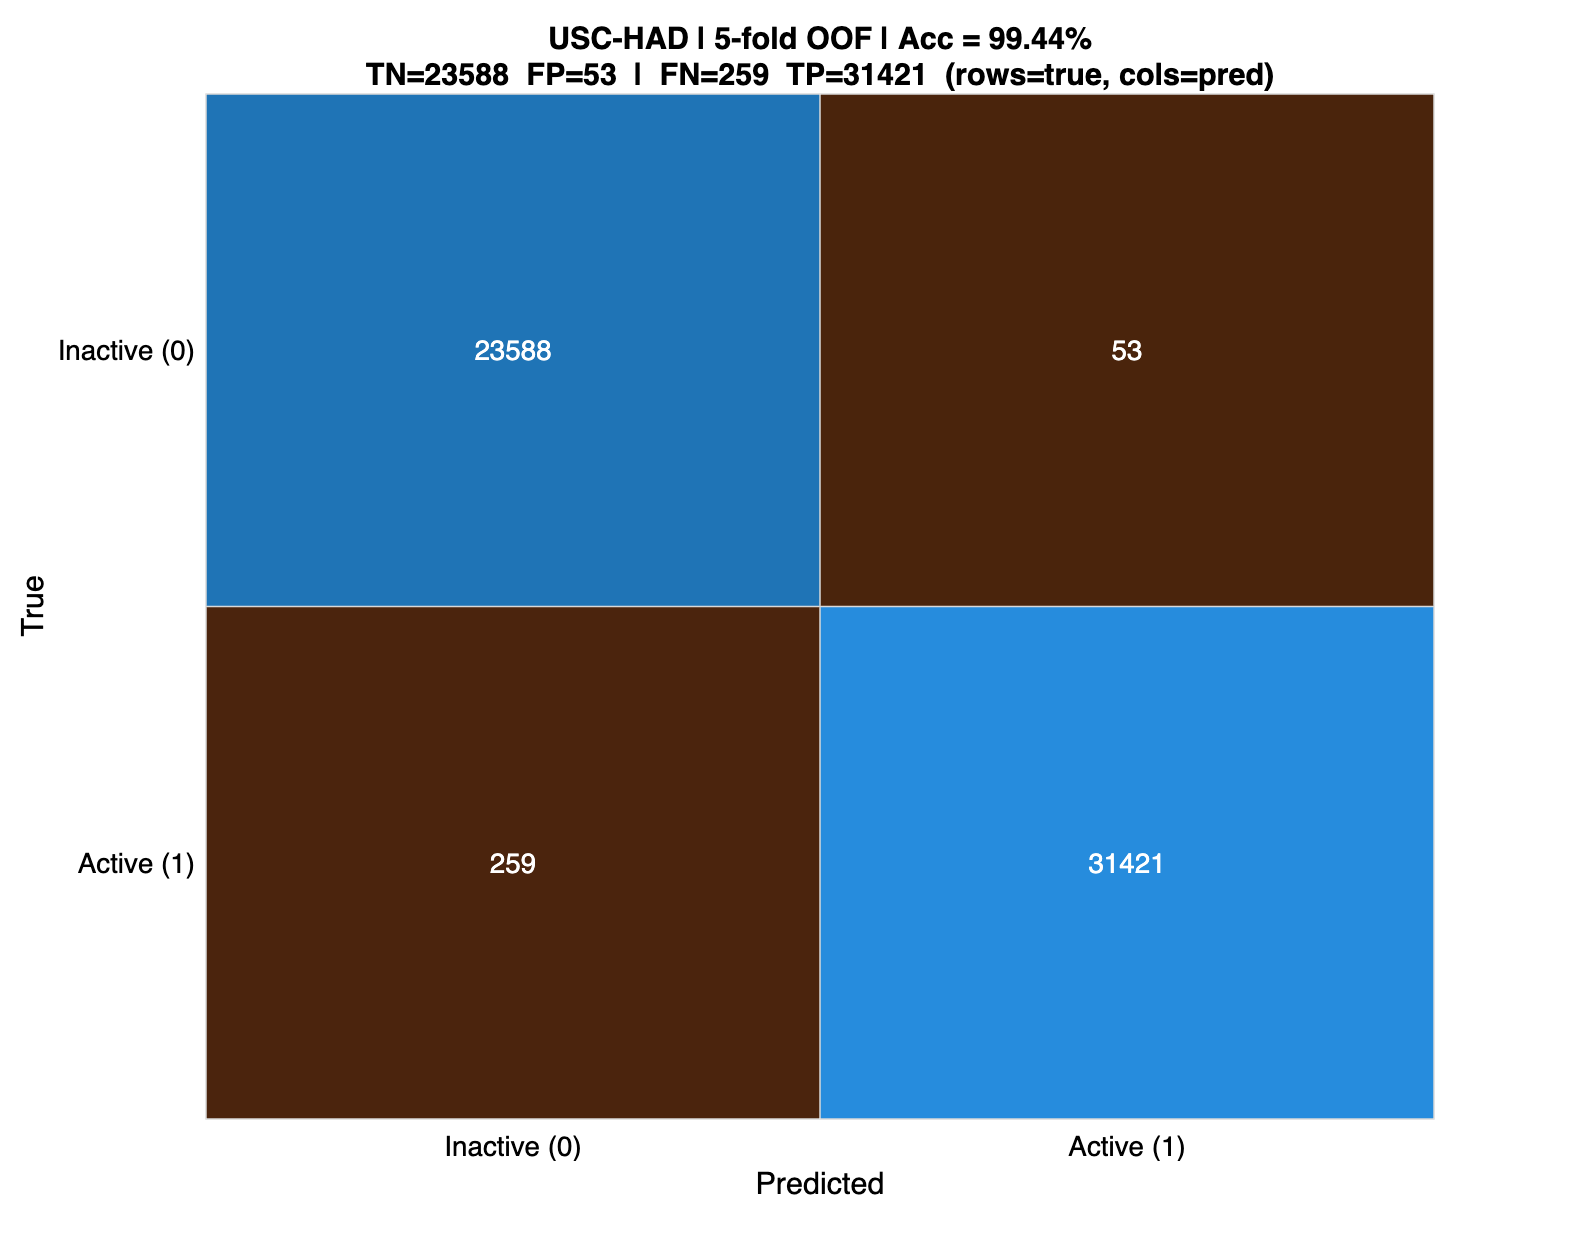
\includegraphics[width=\linewidth,height=0.24\textheight,keepaspectratio]{svm_confusion_matrix_usc_had.png}\\
    \small Binary SVM confusion matrix, USC-HAD.
  \end{minipage}\hfill
  \begin{minipage}[t]{0.48\linewidth}
    \centering
    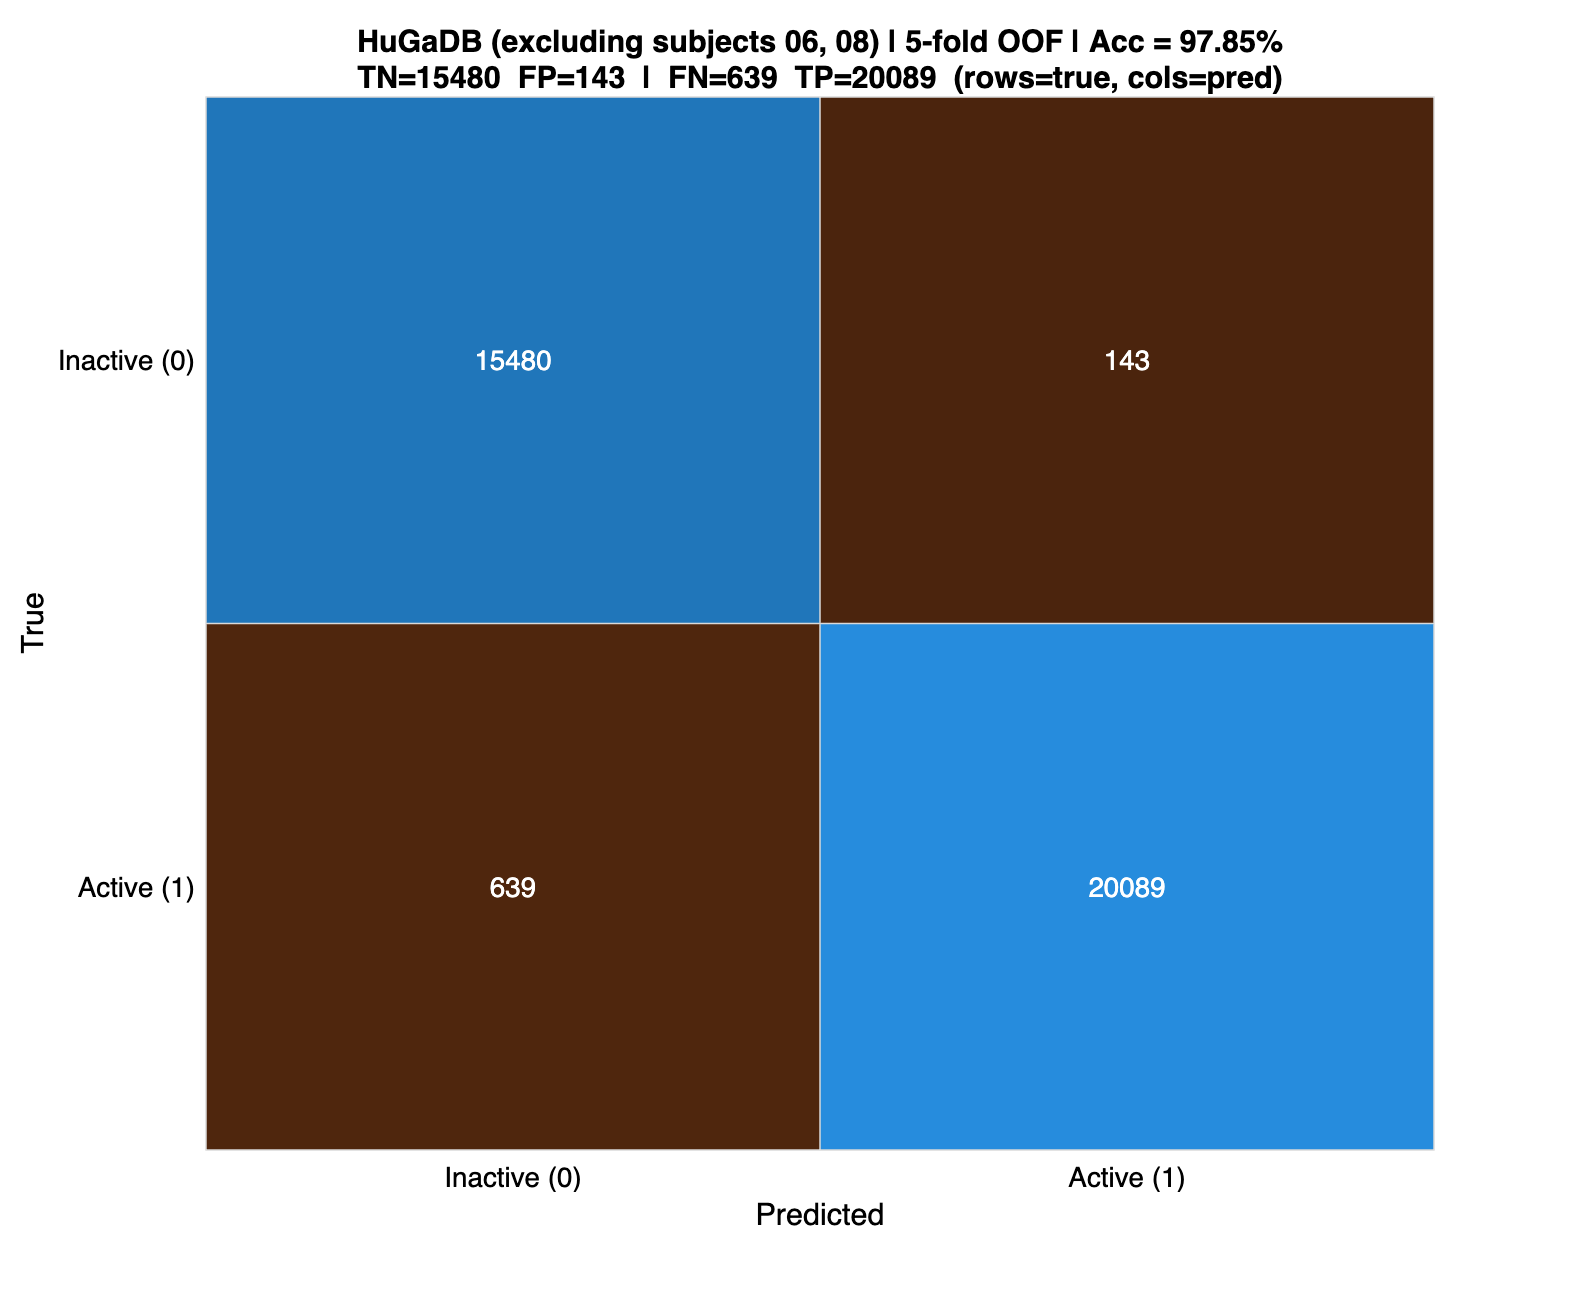
\includegraphics[width=\linewidth,height=0.24\textheight,keepaspectratio]{svm_confusion_matrix_hugadb.png}\\
    \small Binary SVM confusion matrix, HuGaDB.
  \end{minipage}
  \caption{Binary SVM benchmark comparison figures generated by \texttt{RunSvmDatasetAblation}.}
\end{figure}

\begin{figure}[p]
  \centering
  \begin{minipage}[t]{0.48\linewidth}
    \centering
    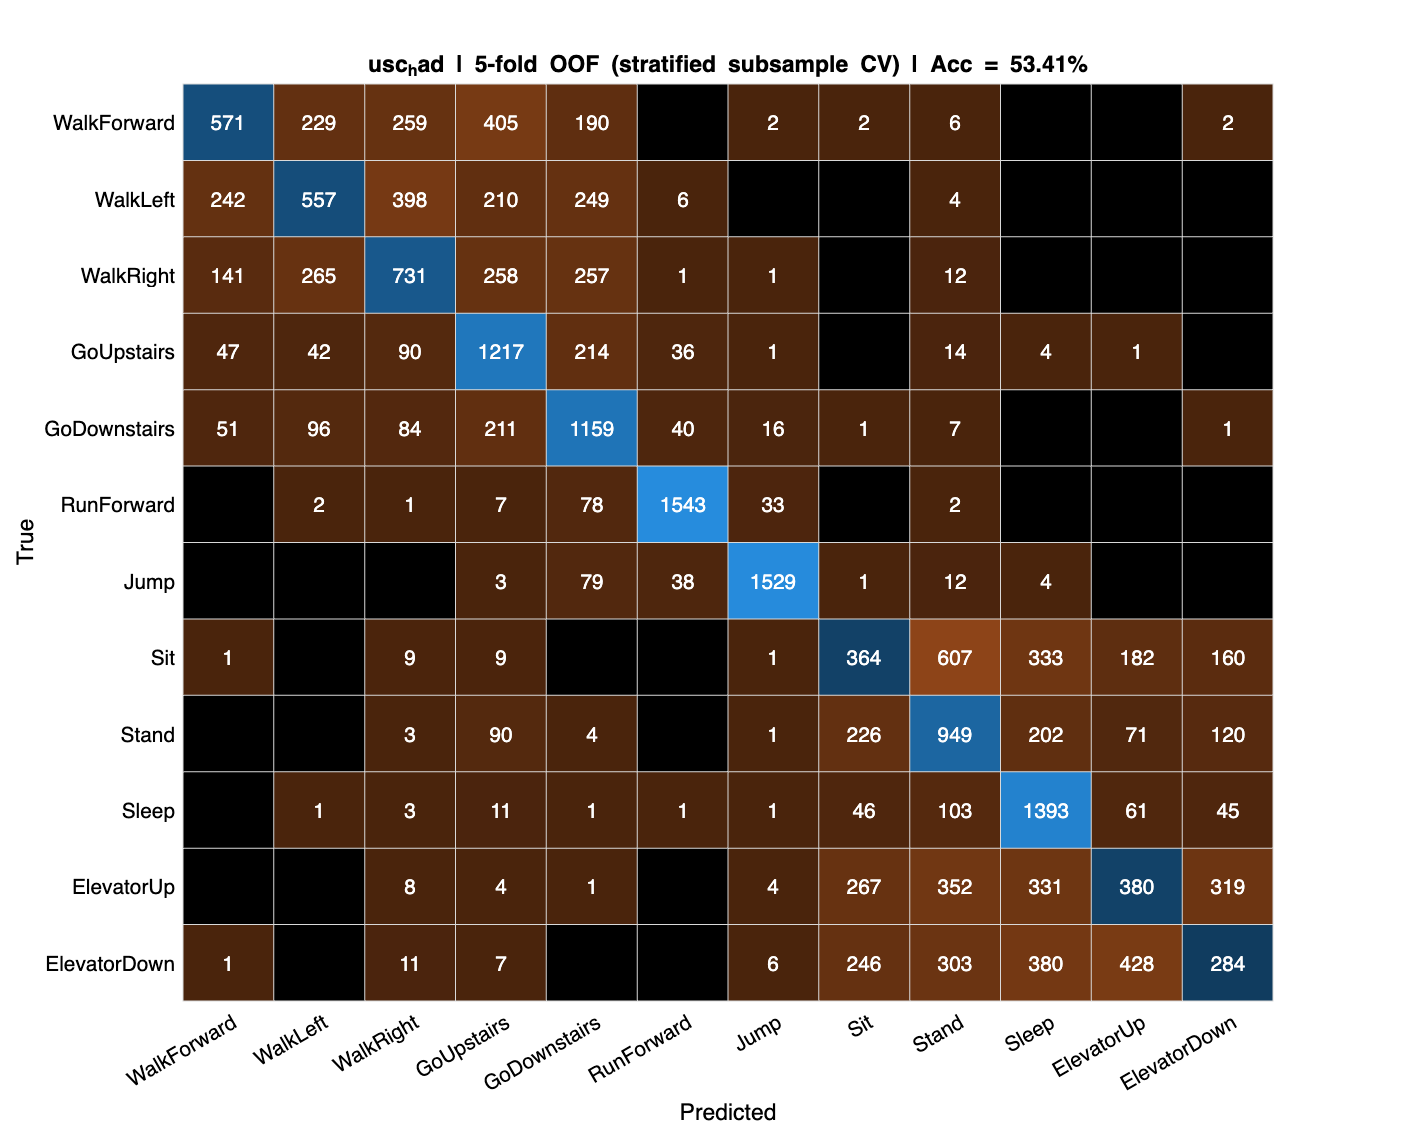
\includegraphics[width=\linewidth,height=0.24\textheight,keepaspectratio]{multiclass_confusion_matrix_usc_had.png}\\
    \small Native multiclass SVM confusion matrix, USC-HAD.
  \end{minipage}\hfill
  \begin{minipage}[t]{0.48\linewidth}
    \centering
    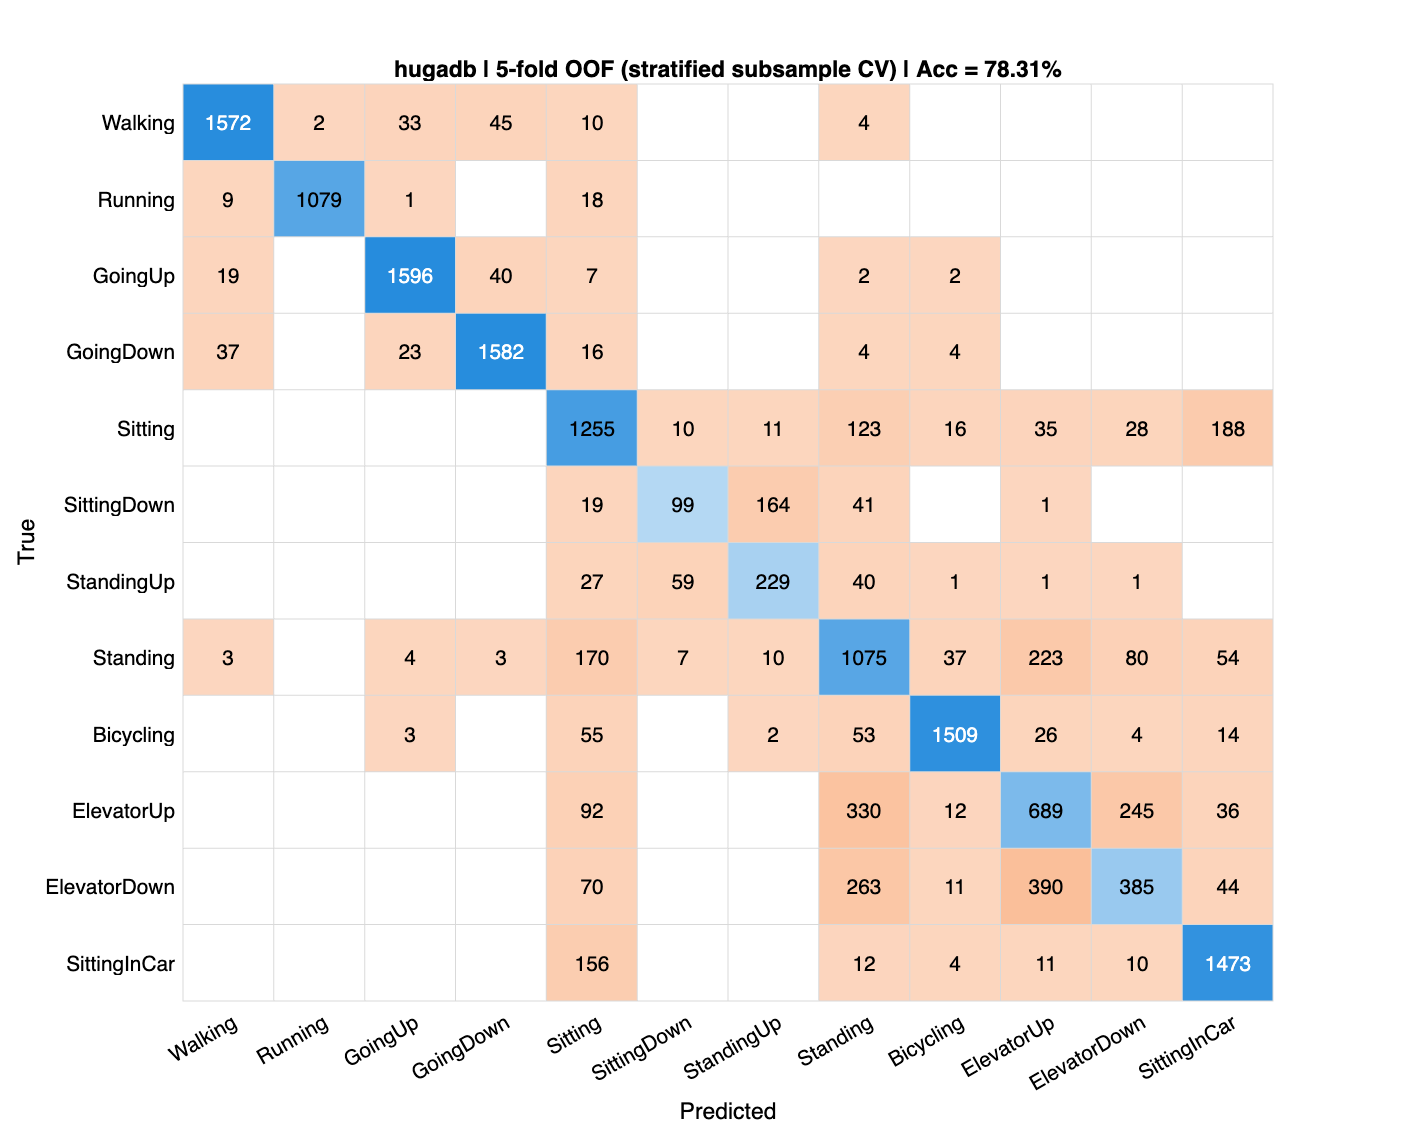
\includegraphics[width=\linewidth,height=0.24\textheight,keepaspectratio]{multiclass_confusion_matrix_hugadb.png}\\
    \small Native multiclass SVM confusion matrix, HuGaDB.
  \end{minipage}
  \caption{Dataset-native multiclass SVM figures generated by \texttt{RunTrainEvalMulticlass}.}
\end{figure}

\begin{figure}[p]
  \centering
  \begin{minipage}[t]{0.48\linewidth}
    \centering
    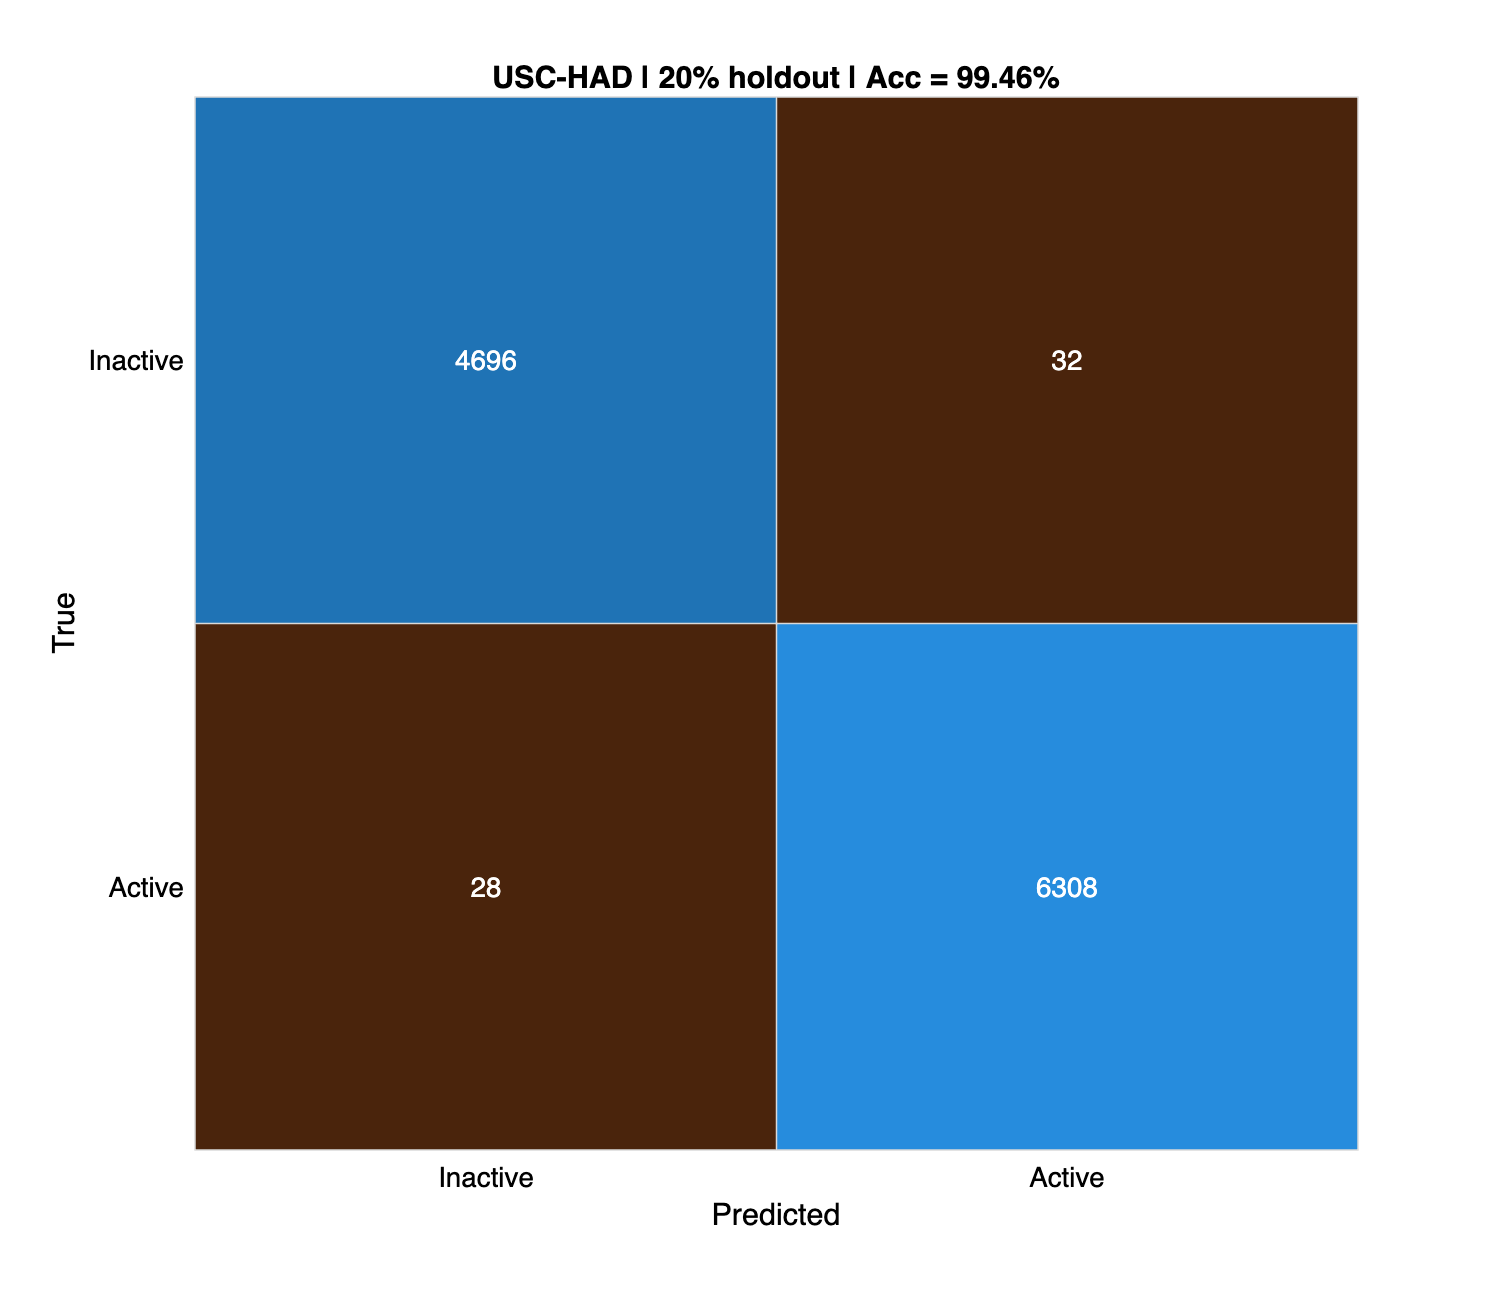
\includegraphics[width=\linewidth,height=0.24\textheight,keepaspectratio]{lstm_confusion_matrix_usc_had.png}\\
    \small Binary LSTM confusion matrix, USC-HAD holdout split.
  \end{minipage}\hfill
  \begin{minipage}[t]{0.48\linewidth}
    \centering
    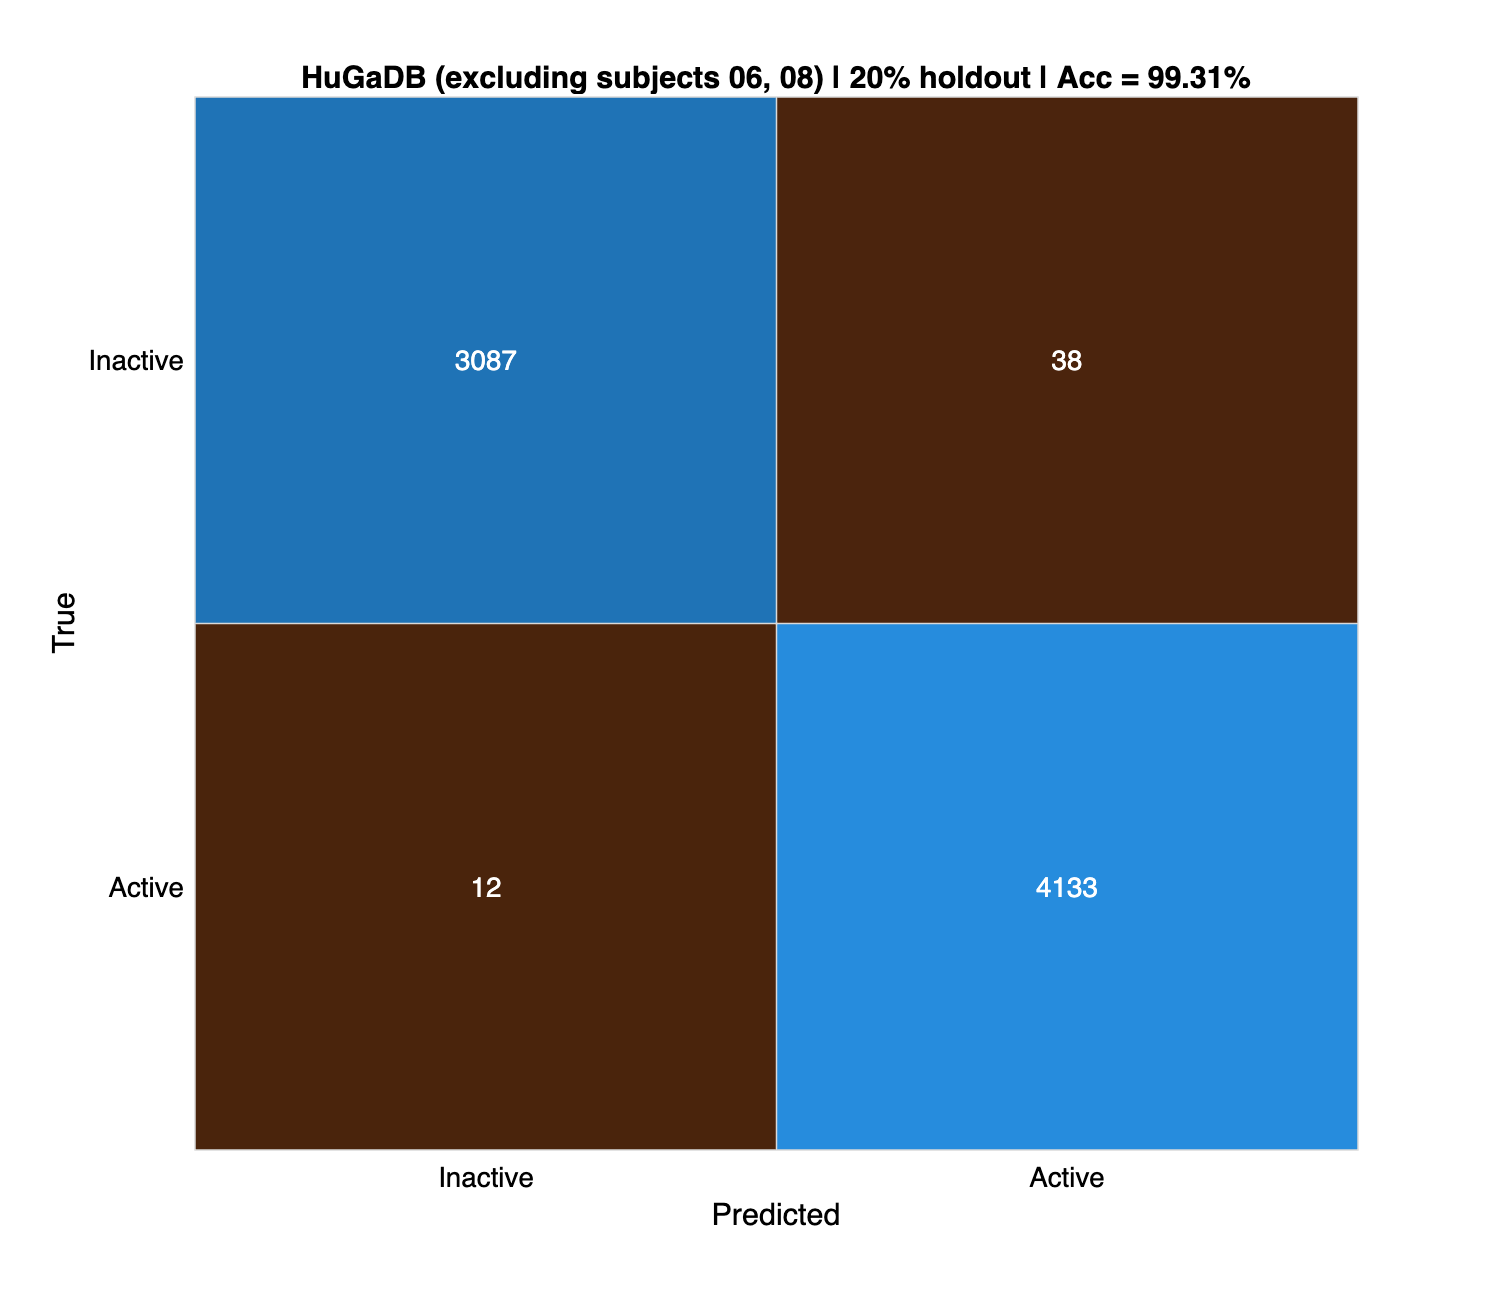
\includegraphics[width=\linewidth,height=0.24\textheight,keepaspectratio]{lstm_confusion_matrix_hugadb.png}\\
    \small Binary LSTM confusion matrix, HuGaDB holdout split.
  \end{minipage}
  \caption{Binary LSTM figures generated by \texttt{RunLstmDatasetAblation}.}
\end{figure}

\begin{figure}[p]
  \centering
  \begin{minipage}[t]{0.48\linewidth}
    \centering
    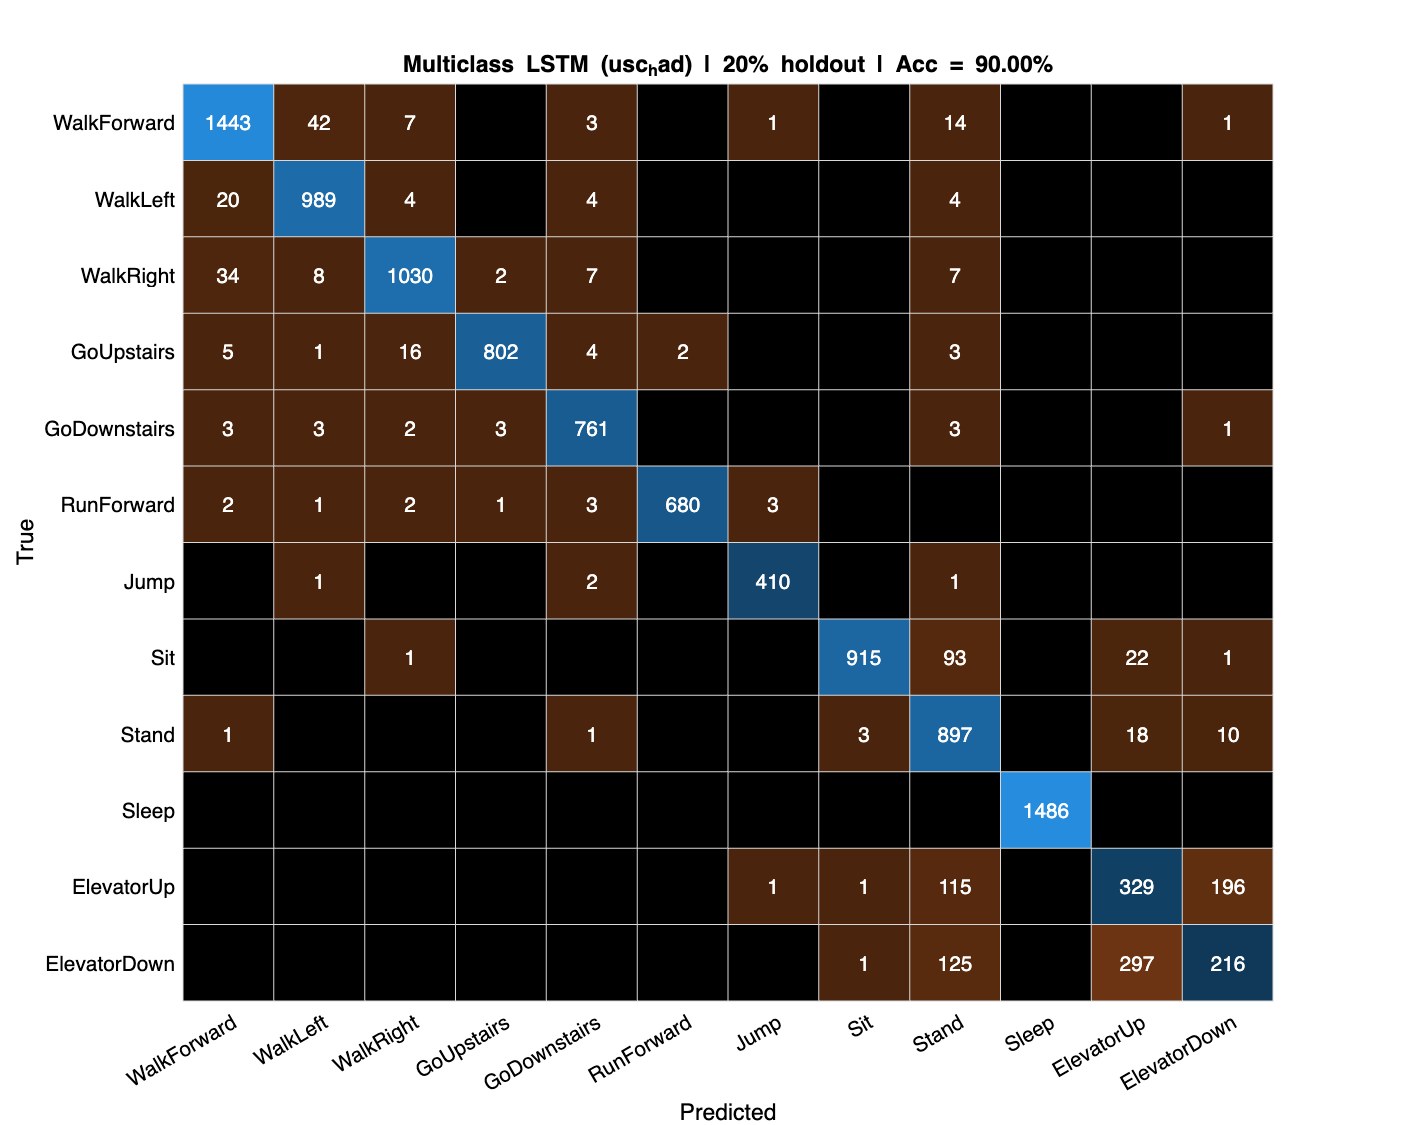
\includegraphics[width=\linewidth,height=0.24\textheight,keepaspectratio]{lstm_multiclass_confusion_matrix_usc_had.png}\\
    \small Native multiclass LSTM confusion matrix, USC-HAD holdout split.
  \end{minipage}\hfill
  \begin{minipage}[t]{0.48\linewidth}
    \centering
    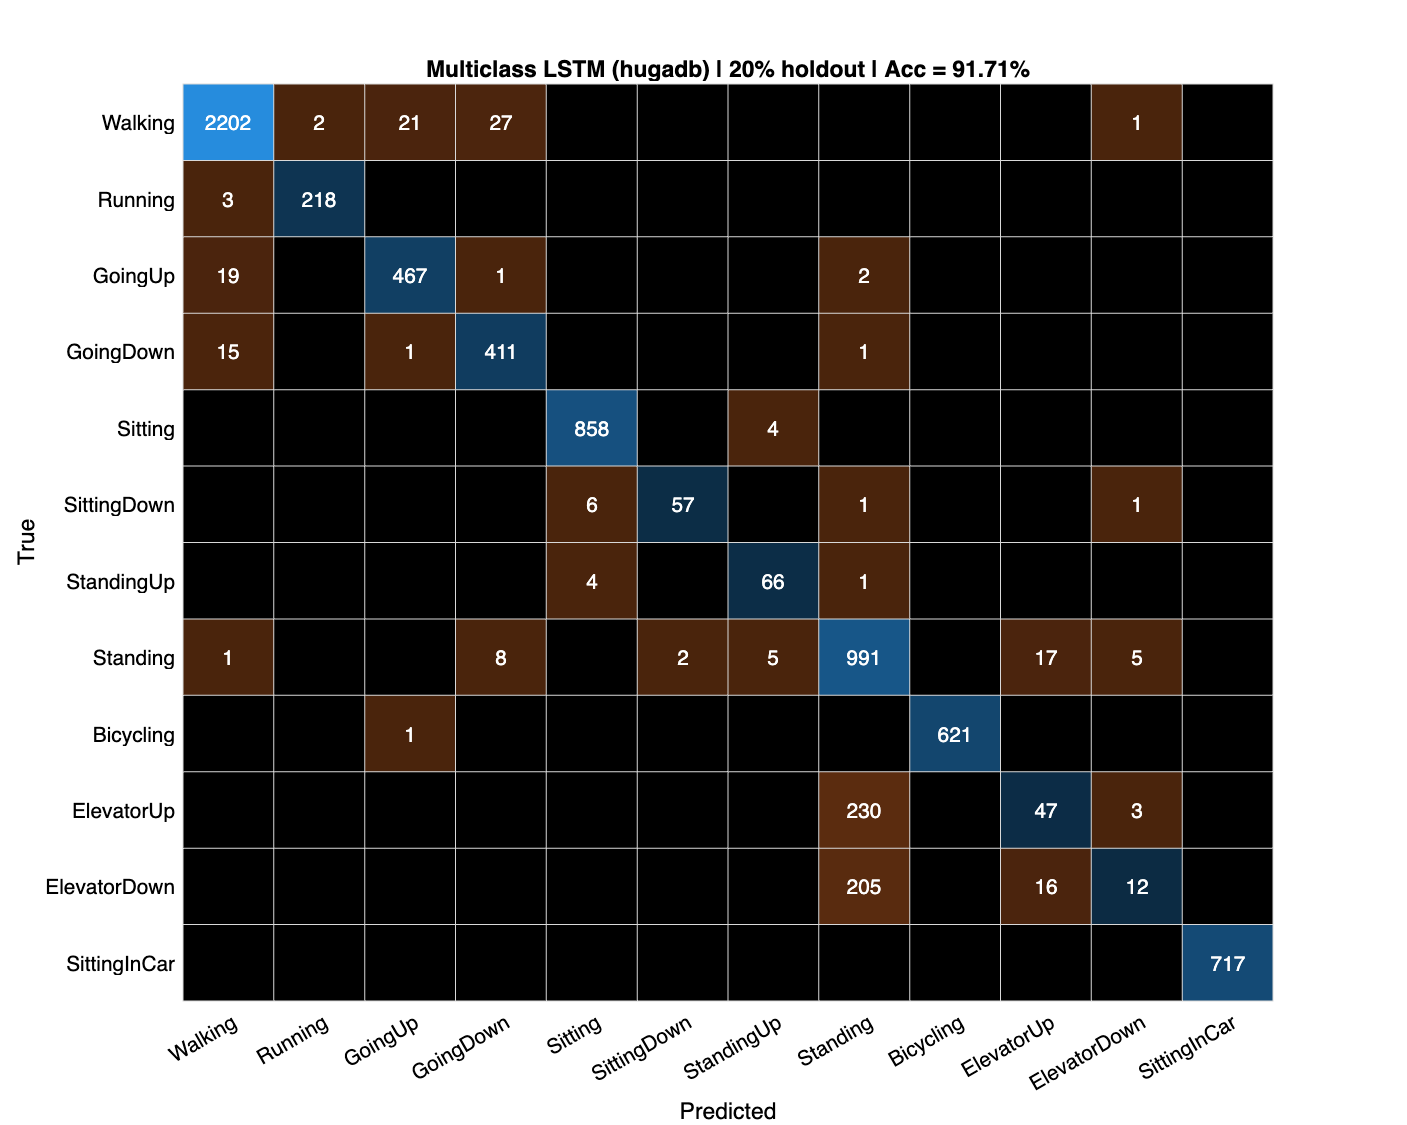
\includegraphics[width=\linewidth,height=0.24\textheight,keepaspectratio]{lstm_multiclass_confusion_matrix_hugadb.png}\\
    \small Native multiclass LSTM confusion matrix, HuGaDB holdout split.
  \end{minipage}
  \caption{Dataset-native multiclass LSTM figures generated by \texttt{RunTrainEvalLstmMulticlass}.}
\end{figure}

\begin{figure}[p]
  \centering
  \begin{minipage}[t]{0.48\linewidth}
    \centering
    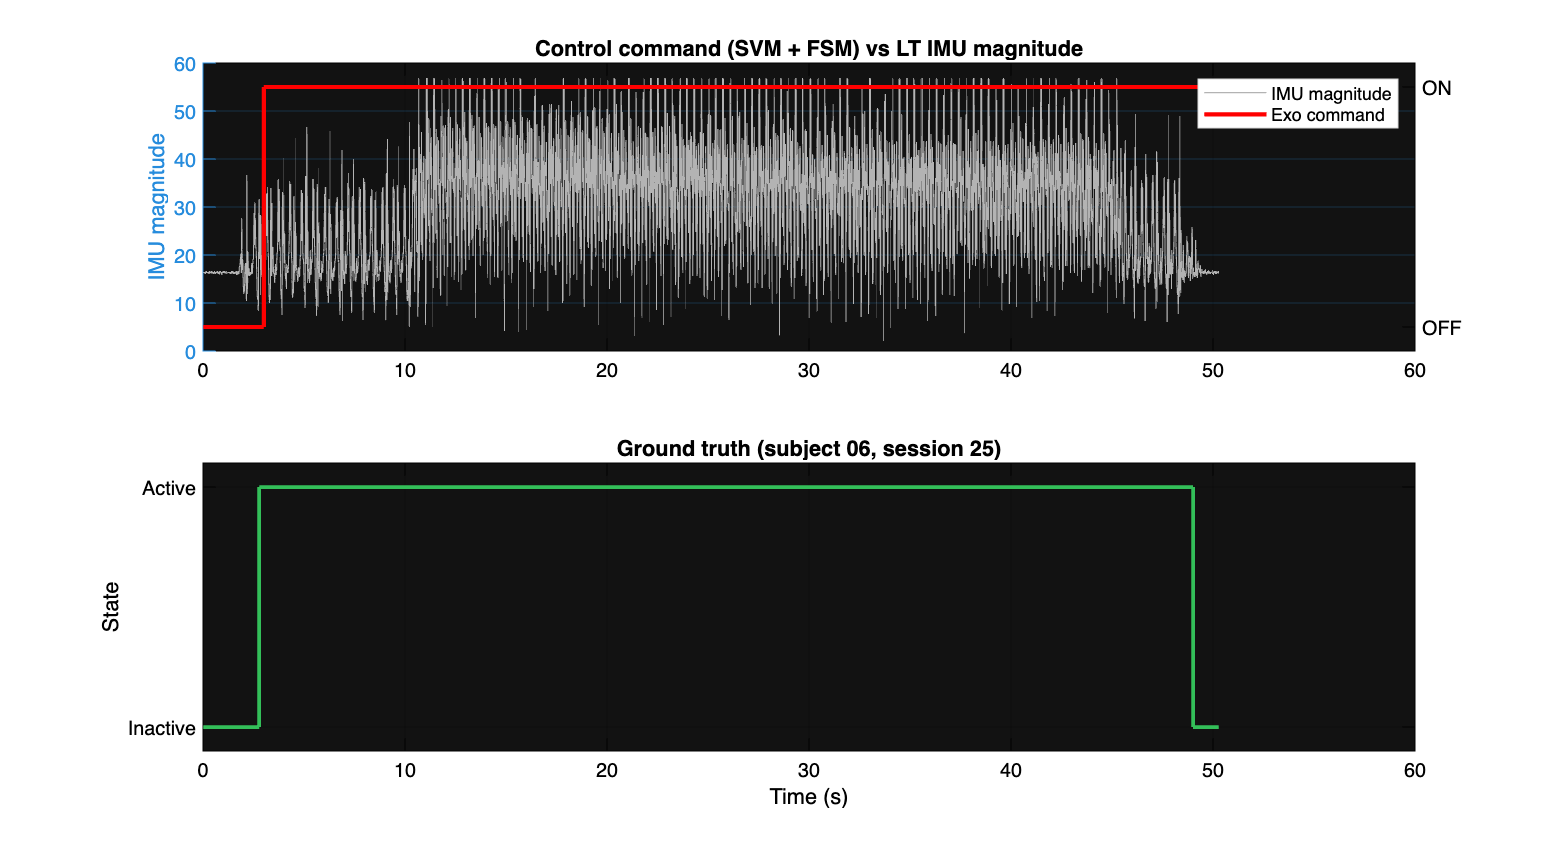
\includegraphics[width=\linewidth,height=0.24\textheight,keepaspectratio]{pipeline_binary_svm_output.png}\\
    \small Binary SVM replay pipeline on held-out HuGaDB data.
  \end{minipage}\hfill
  \begin{minipage}[t]{0.48\linewidth}
    \centering
    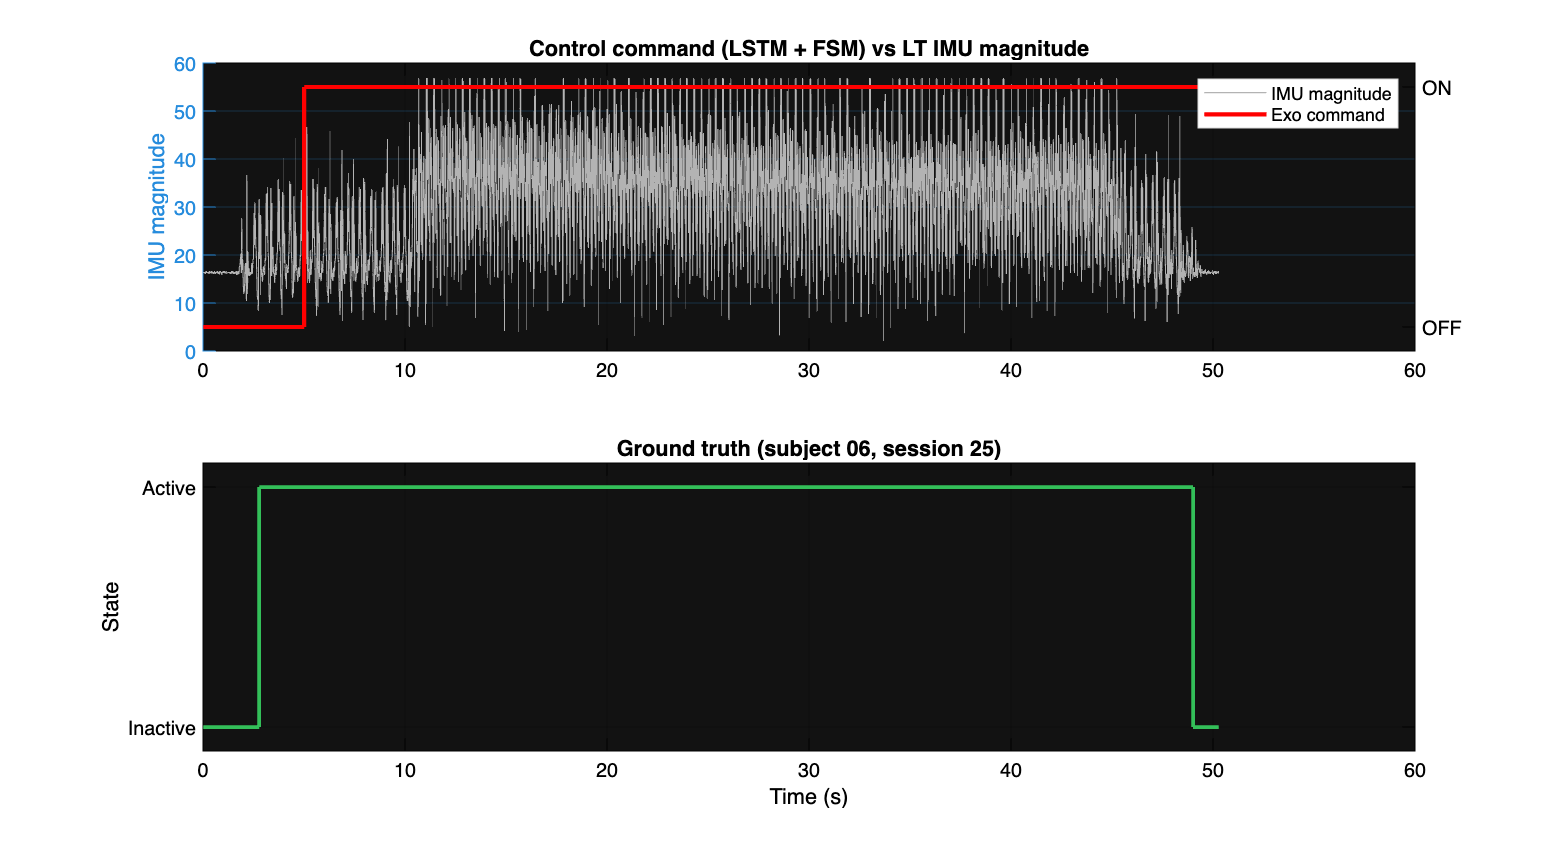
\includegraphics[width=\linewidth,height=0.24\textheight,keepaspectratio]{pipeline_output_lstm.png}\\
    \small Binary LSTM replay pipeline on held-out HuGaDB data.
  \end{minipage}
  \caption{Replay-pipeline figures generated by the binary SVM and binary LSTM scripts.}
\end{figure}

\begin{figure}[p]
  \centering
  \begin{minipage}[t]{0.65\linewidth}
    \centering
    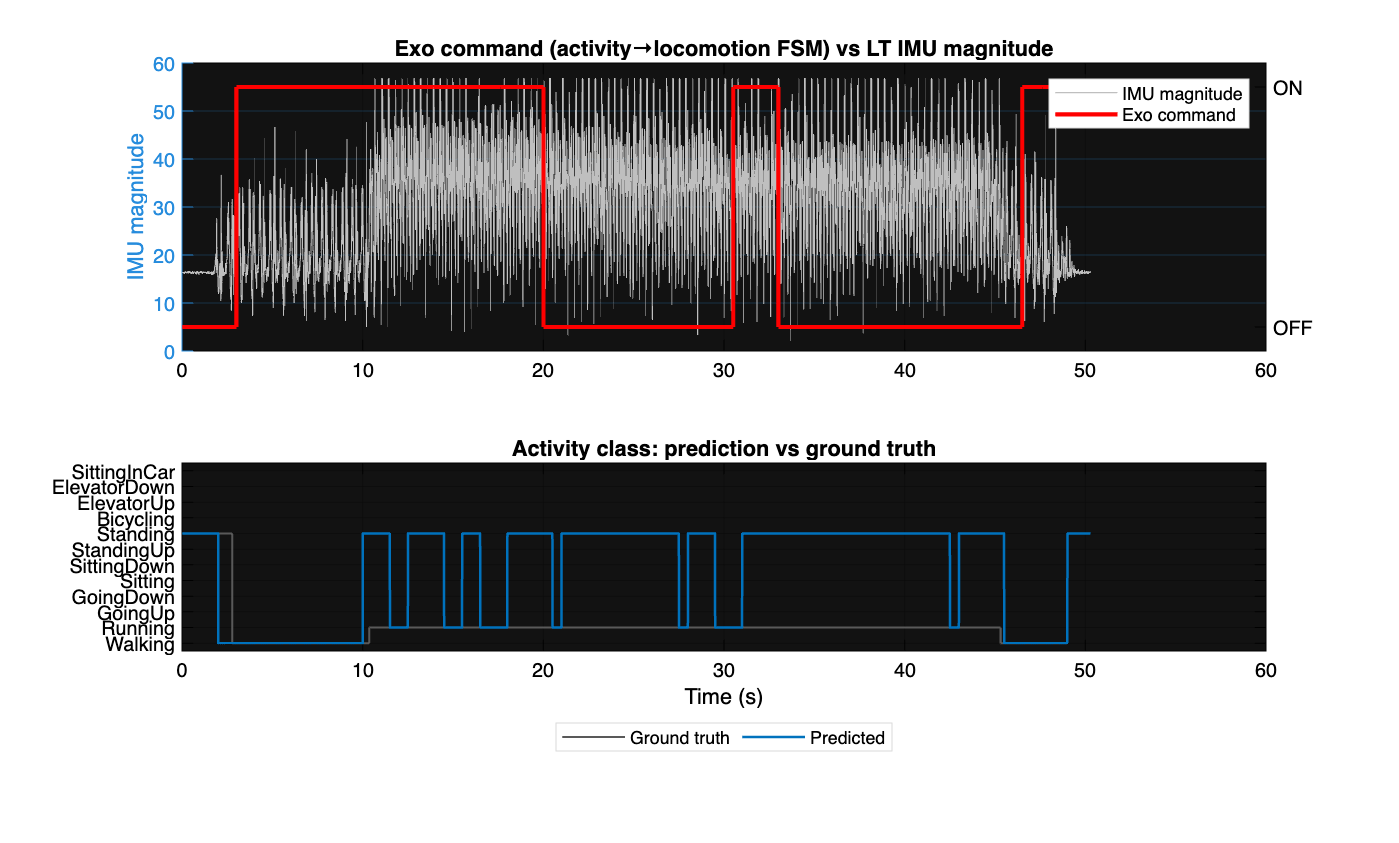
\includegraphics[width=\linewidth,height=0.24\textheight,keepaspectratio]{pipeline_multiclass_output.png}\\
    \small Multiclass SVM replay pipeline on held-out HuGaDB data.
  \end{minipage}
  \caption{Additional replay-pipeline figure generated by the multiclass SVM script.}
\end{figure}

\clearpage
\section{Overall Interpretation}
Taken together, the results show that the project has successfully delivered a reproducible software baseline for exoskeleton assist gating. The final repository now separates benchmark comparison from the actual deployment path: USC-HAD and HuGaDB are evaluated separately for comparison evidence, while the active binary SVM pipeline is based on HuGaDB and reserves subjects 06 and 08 for simulation. The Kalman and FSM blocks remain integrated into an end-to-end control flow, and the report metrics are traceable to versioned MATLAB outputs. At the same time, the discussion also makes clear what remains unfinished: subject-specific tuning, truly predictive transition detection, hardware deployment, and controlled user validation under realistic load-transport tasks.

\section{Visualization Tools and Software Architecture}
Real-time visualization is integrated in MATLAB through scripts such as \texttt{RunExoskeletonPipeline.m}.

The codebase uses per-script path resolution, a modular \path{src/} tree for acquisition, fusion, classification, and features, and \path{docs/System_Design.md} for architecture documentation. Repository: \url{https://github.com/Rex-Yim/AutomationForExoskeleton}.


\chapter{Conclusions and Future Work}
% Chapter 5: interim PDF remaining work + timeline + risks + repository status
\section{Remaining tasks and roadmap (from interim report, Jan 2026)}
The following items were listed in the original submission as work remaining toward completion:
\begin{itemize}
  \item \textbf{Intention detection:} Optional LSTM baseline exists in-repo; further work on multi-mode transitions, speed variations, and SVM+LSTM ensembles; pursue $>90$\% accuracy via domain-specific tuning.
  \item \textbf{Machine learning deployment:} Deploy trained SVM/LSTM models for terrain recognition on embedded targets; extend confusion-matrix reporting; add embedded deployment scripts (MATLAB Coder).
  \item \textbf{Hardware integration:} Deploy validated control software onto the ExoTechHK microcontroller.
  \item \textbf{Testing and validation:} Bench tests, ethical user trials with torque limits, performance evaluation (accuracy, confusion matrix, precision, recall).
  \item \textbf{Documentation and presentation:} Final report, slides, video demonstration, comparative literature benchmarks.
\end{itemize}

\section{Future work beyond the FYP (interim PDF)}
\begin{itemize}
  \item \textbf{Personalization:} Short calibration walks with transfer learning and lightweight RL (e.g., PPO/SAC) to tune assistance.
  \item \textbf{Injury-risk assessment:} Integrate ergonomic risk frameworks such as Zelik et al.~\cite{zelik2022} into user trials.
\end{itemize}

\section{Project timeline (interim PDF)}
Table~\ref{tab:timeline} reproduces the phased plan from the Jan 2026 report (notional dates; confirm with your advisor).

\begin{table}[htbp]
  \centering
  \small
  \caption{Phased development plan (interim submission).}
  \label{tab:timeline}
  \begin{tabular}{@{}p{2.7cm}p{2.3cm}p{4.4cm}p{4.4cm}@{}}
    \toprule
    \textbf{Phase} & \textbf{Duration} & \textbf{Key activities} & \textbf{Milestones} \\
    \midrule
    ML training \& simulation integration & Jan -- Feb 2026 (2 months) & Train/deploy ML; Simulink HIL-style virtual tests; locomotion modes under load & Validated models ($\geq 90$\% target); simulation demo \\
    Hardware integration \& testing & Mar -- Apr 15, 2026 (1.5 months) & Software--hardware integration; bench and limited treadmill tests (5--10 trials); ethics & Logs with latency/error metrics \\
    Optimization, documentation, finalization & Apr 16 -- May 2026 (1.5 months) & Refine from tests; compile report; presentation & Submitted report; presentation; archived repository \\
    \bottomrule
  \end{tabular}
\end{table}

\section{Risk assessment (interim PDF)}
Table~\ref{tab:risks} summarizes risks and mitigations from the Jan 2026 report.

\begin{table}[htbp]
  \centering
  \small
  \caption{Risks and mitigations (interim submission).}
  \label{tab:risks}
  \begin{tabular}{@{}p{3.6cm}ccp{5.5cm}@{}}
    \toprule
    \textbf{Risk} & \textbf{Like.} & \textbf{Imp.} & \textbf{Mitigation} \\
    \midrule
    Hardware integration delays (e.g., actuator vs.\ ExoTechHK frame) & M & H & Modular COTS parts; parallel software; early prototype access \\
    ML underperformance ($<85$\% accuracy) & L & M & Rule/ML hybrid fallback; partner datasets; cross-validation / RL tuning \\
    Trial delays & M & H & Public/simulated data interim; limit volunteers; secure IRB early \\
    Budget overrun & L & L & University funding; HKSTP supplements \\
    \bottomrule
  \end{tabular}
\end{table}

\section{Repository status (consolidated, 2026)}
Relative to the interim plan, the following are \textbf{delivered in software}: Kalman fusion baseline; binary RBF SVM with merged USC-HAD+HuGaDB training and dataset ablation scripts; optional twelve-class ECOC SVM; optional binary LSTM sequence classifier (\texttt{TrainLstmBinary}, \texttt{EvaluateLstmConfusion}, \texttt{RunExoskeletonPipelineLstm}); asymmetric FSM; documentation and evaluation figures.

\textbf{Not delivered:} hybrid SVM+LSTM fusion as in the original pseudocode, MATLAB Coder deployment, ROS/PID torque layer, hardware controller integration, and prospective user trials---these remain aligned with the roadmap and risk tables above.

\textbf{Synthesis:} The LaTeX report intentionally preserves the \textbf{full interim narrative} (objectives, proposed LSTM/EKF/ROS extensions, timeline, risks) while adding a \textbf{faithful description of the implemented repository}, so readers can distinguish planned scope from validated baseline.


\clearpage
% IEEE reference list: IEEEtran bibliography style (IEEE Reference Style).
\chapter*{References}
\addcontentsline{toc}{chapter}{References}
\bibliographystyle{IEEEtran}
\bibliography{references}


\end{document}
